\documentclass[12pt,t]{beamer}
% \documentclass[t]{beamer}
\usepackage[utf8]{inputenc}
\usepackage[catalan]{babel}
\usepackage{verbatim}
\usepackage{hyperref}
\usepackage{amsfonts,amssymb,amsmath,amsthm, wasysym, multirow}
\usepackage{listings}
\usepackage[T1]{fontenc}        
\usepackage{pgf}
\usepackage{epsdice}
\usepackage{pgfpages}
\usepackage{tikz}

\usepackage{pgfpages}
\pgfpagesuselayout{4 on 1}[a4paper,border shrink=5mm,landscape]
\setbeamertemplate{footline}[frame number]
%\usetikzlibrary{arrows,shapes,plotmarks,backgrounds,trees,positioning}
%\usetikzlibrary{decorations.pathmorphing,calc,snakes}
%\usepackage{marvosym}
%
\usetheme[hideothersubsections,left]{Marburg}
\usecolortheme{sidebartab}
\useinnertheme[shadow]{rounded}
% \useoutertheme[footline=empty,subsection=true,compress]{infolines}
% \useoutertheme[footline=empty,subsection=true,compress]{miniframes}
% \usefonttheme{serif}

\setbeamertemplate{caption}[numbered]
\setbeamertemplate{navigation symbols}{}


\newcommand{\red}[1]{\textcolor{red}{#1}}
\newcommand{\green}[1]{\textcolor{green}{#1}}
\newcommand{\blue}[1]{\textcolor{blue}{#1}}
\newcommand{\gray}[1]{\textcolor{gray}{#1}}
\renewcommand{\emph}[1]{{\color{red}#1}}

\setbeamertemplate{frametitle}
{\begin{centering}
\medskip
\color{blue}
\textbf{\insertframetitle}
\medskip
\end{centering}
}
\usecolortheme{rose}
\usecolortheme{dolphin}
\mode<presentation>


\newcommand{\CC}{\mathbb{C}}
\newcommand{\RR}{\mathbb{R}}
\newcommand{\ZZ}{\mathbb{Z}}
\newcommand{\NN}{\mathbb{N}}
\newcommand{\KK}{\mathbb{K}}
\newcommand{\MM}{\mathcal{M}}
%\newcommand{\dbinom}{\displaystyle\binom}

\newcommand{\limn}{{\displaystyle \lim_{n\to\infty}}}
\renewcommand{\leq}{\leqslant}
\renewcommand{\geq}{\geqslant}
\def\tendeix{{\displaystyle\mathop{\longrightarrow}_{\scriptscriptstyle
n\to\infty}}}

\newcommand{\matriu}[1]{\left(\begin{matrix} #1 \end{matrix}\right)}

% \newcommand{\qed}{\hbox{}\nobreak\hfill\vrule width 1.4mm height 1.4mm depth 0mm
%     \par \goodbreak \smallskip}
%
% %
\theoremstyle{plain}
\newtheorem{teorema}{Teorema}
\newtheorem{prop}{Proposició}
\newtheorem{cor}{Coro\l.lari}
\theoremstyle{definition}
\newtheorem{exemple}{Exemple}
\newtheorem{defin}{Definició}
\newtheorem{obs}{Observació}

\newcounter{seccions}
\newcommand{\seccio}[1]{\addtocounter{seccions}{1}
\medskip\par\noindent\emph{\theseccions.
#1}\smallskip\par }

\newcommand{\EM}{\Omega}
\newcommand{\PP}{\mathcal{P}}

\title[\red{Matemàtiques II}]{}
\author[]{}
\date{}



\begin{document}
\beamertemplatedotitem

\lstset{backgroundcolor=\color{green!50}}
\lstset{breaklines=true}
\lstset{basicstyle=\ttfamily}


\section{Diagnòstics: Estudi dels residus}

\begin{frame}
\vfill
\begin{center}
\gray{\LARGE Anàlisi de Residus}
\end{center}
\vfill
\end{frame}

\begin{frame}{Hipòtesis del model de regressió lineal}

L'estimació i inferència a partir del model de regressió lineal depèn de diverses hipòtesis, que hauran de ser comprovades emprant \emph{diagnòstics de regressió}. Els problemes potencials es classifiquen en tres categories:

\begin{enumerate}
\item \emph{Errors}: Els errors han de seguir una $N(0,\sigma)$, amb la mateixa variància, i ser incorrelats.

\item \emph{Model}: Els punts s'han d'ajustar a l'estructura lineal considerada.

\item \emph{Observacions anòmales}: De vegades unes quantes observacions no s'ajusten al model.
\end{enumerate}

\end{frame}

\begin{frame}{Tipus de diagnòstics de regressió}

Els diagnòstics poden ser:
\begin{itemize}
\item \emph{gràfics}: Més flexibles però més difícils d'interpretar $\Rightarrow$ Lliçó 28 de R.
\item \emph{numèrics}: D'utilitat més limitada però amb interpretació immediata.
\end{itemize}

\end{frame}

\subsection{Distribució dels errors}
\begin{frame}[fragile]{Variància no constant}

Un dels problemes que pot patir el nostre model és que la variància dels residus no sigui constant. Vegem-ne un exemple

\begin{verbatim}
> x<-runif(100)
> y<-1-2*x+0.3*x*rnorm(100)
> par(mfrow=c(1,2))
> plot(x,y)
> r=lm(y~x)
> abline(r,col="red")
> plot(r$res~r$fitted.values)
\end{verbatim}

\end{frame}

\begin{frame}[fragile]{Variància no constant}
\begin{center}
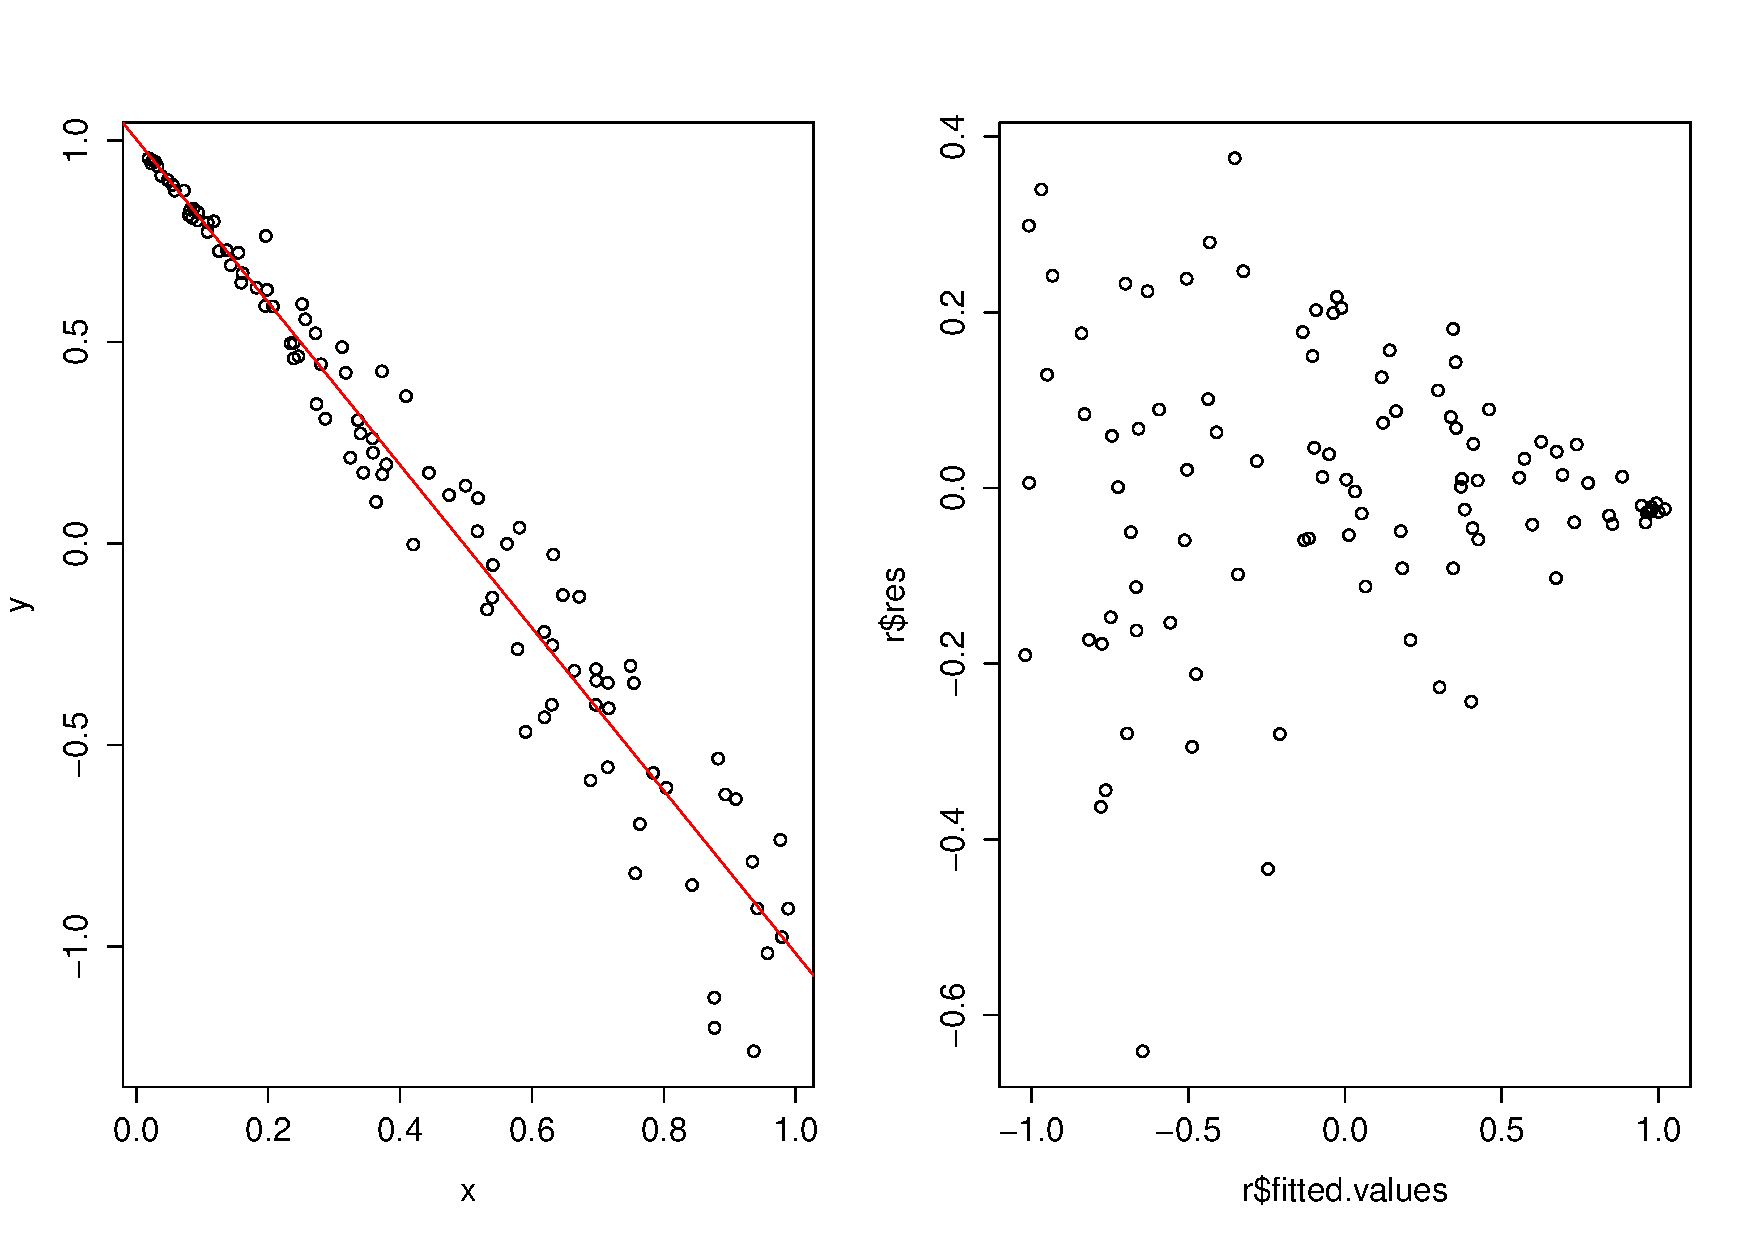
\includegraphics[scale=0.35]{hetero.pdf}
\end{center}
\end{frame}

\begin{frame}{Variància no constant}

En el cas que la variància no sigui constant, direm que el model presenta \emph{heteroscedasticitat}.

\vspace{0.25cm}

Gràficament es pot comprovar amb el gràfic $\{(\hat{y}_i,e_i)\}_{i=1,\ldots,n}$, detectant zones sense punts.

\vspace{0.25cm}

Emperò també disposam de tests per contrastar-ho.

\end{frame}

\begin{frame}{Test de White}
\begin{enumerate}
\item Obtenim els residus $\{e_i\}_{i=1,\ldots,n}$  de la regressió lineal inicial.
\item Calculam el $R^2$ de la regressió lineal dels $e_i^2$ respecte de les variables inicials, els seus quadrats i els productes creuats dos a dos.
\item Obtenim l'estadístic $X_0=nR^2$, el qual, suposant que la variància és constant, segueix una $\chi^2_q$, on $q$ és el número de variables independents de la regressió del pas anterior.
\item Calculam el p-valor 
$$P(\chi_q^2\geq X_0)$$
 amb el significat usual.
\end{enumerate}
\end{frame}

\begin{frame}[fragile]{Test de White}
Anem a aplicar-lo a l'exemple anterior.

\begin{verbatim}
> residus=r$res
> X0=length(residus)*
  summary(lm(residus^2~x+x^2))$r.squared
> 1-pchisq(X0,2)
[1] 0.0006494604
\end{verbatim}

I per tant, podem rebutjar la hipòtesi nul·la i concloure que el model presenta heteroscedasticitat. Amb R, es pot emprar la funció \texttt{white.test} del paquet \texttt{bstats}.
\begin{footnotesize}
\begin{verbatim}
> install.packages("bstats")
> library(bstats)
> r<-lm(y~x)
> white.test(r)
	White test for constant variance
data:  
White = 14.6983, df = 2, p-value = 0.0006431
\end{verbatim}
\end{footnotesize}

\end{frame}

\begin{frame}[fragile]{Normalitat}
Com ja hem vist anteriorment, els residus han de seguir una distribució $N(0,\sigma)$ variància constant. Això es pot comprovar amb el test KS, emprant $S^2$ com estimador de la variància. 

\vspace{0.25cm}

També es pot recórrer a l'histograma o al gràfic QQ-plot.

\begin{verbatim}
> ks.test(r$res,"pnorm",0,summary(r)$sigma)
	One-sample Kolmogorov-Smirnov test
data:  r$res
D = 0.136, p-value = 0.04958
alternative hypothesis: two-sided
> library(car)
> qqPlot(r$res,"norm")
\end{verbatim}

Tots dos criteris rebutgen la normalitat dels residus del nostre exemple.
\end{frame}



\begin{frame}[fragile]{Normalitat}

\begin{center}
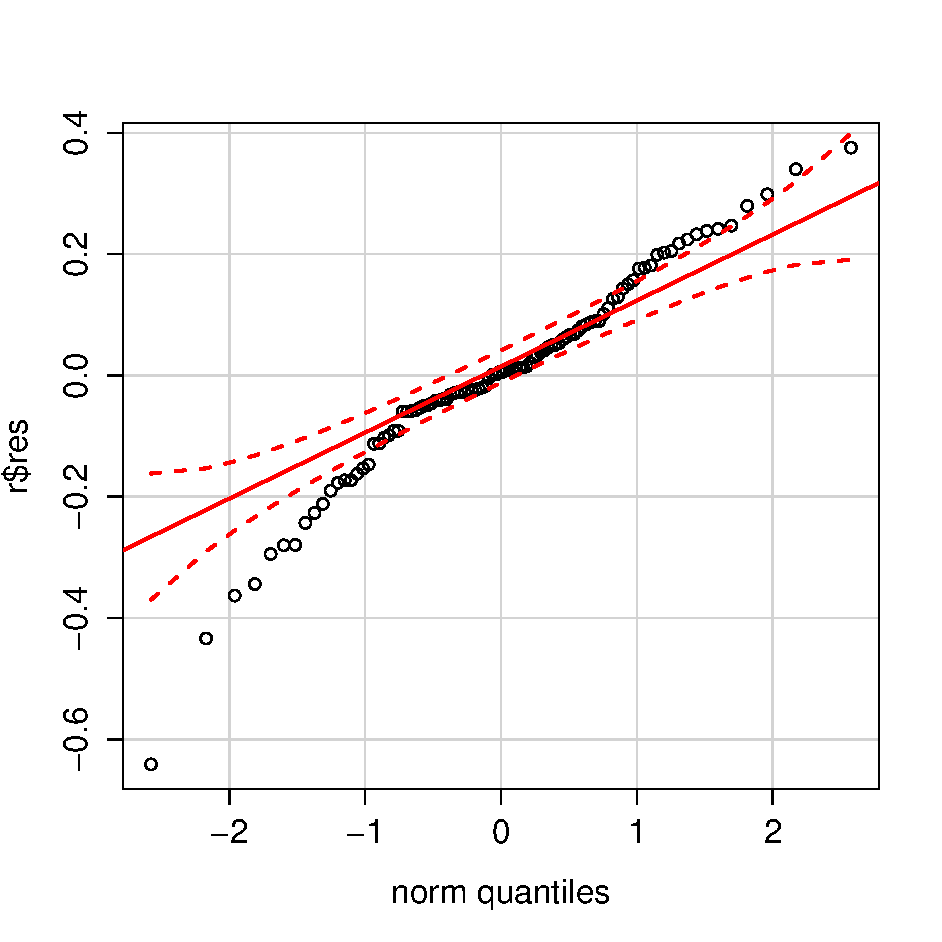
\includegraphics[scale=0.5]{qqPlot.pdf}
\end{center}


\end{frame}

\begin{frame}{Correlació dels residus: Test de Durbin-Watson}
Els residus han de ser incorrelats. L'autocorrelació pot ser de dos tipus:
\begin{itemize}
\item \emph{Autocorrelació positiva}: Un valor positiu (negatiu) d'un error genera una successió de residus positius (negatius).
\item \emph{Autocorrelació negativa}: Els residus van alternant de signe. 
\end{itemize}
Per comprovar si es satisfà que els residus no presenten correlació, es pot aplicar el test de \emph{Durbin-Watson}.

\end{frame}

\begin{frame}{Correlació dels residus: Test de Durbin-Watson}
Siguin $\{e_i\}_{i=1,\ldots,n}$ els residus de la regressió. Siguin $E_i$ i $E_{i-1}$ les variables aleatòries error (traslladades en un índex) i $E_i=\beta_1E_{i-1}+\beta_0$ la recta de regressió de $E_i$ respecte a $E_{i-1}$. Es planteja el següent contrast:
$$\left\{\begin{array}{ll} H_0: \beta_1=0,\\H_1: \beta_1\neq0\end{array}\right.$$
Aleshores es defineix el següent estadístic de contrast
$$d=\frac{\sum^n_{i=2}{(e_i-e_{i-1})^2}}{\sum_{i=1}^n{e_i^2}}$$
El valor d'aquest estadístic és aproximadament $2(1-b_1)$ on $b_1$ és una estimació de $\beta_1$. Si $H_0$ és certa, la seva distribució és la d'una certa combinació lineal de $\chi^2$. 
\end{frame}

\begin{frame}{Test de Durbin-Watson}
El test necessita d'una taula de valors crítics per prendre la decisió final. En concret, $d$ s'ha de comparar amb dos valors crítics $d_{L,\alpha}$ i $d_{U,\alpha}$ on $\alpha$ és el nivell de significació que depenen de $n$ i de $k$.

\vspace{0.25cm}
Contrastem si hi ha autocorrelació positiva
\begin{itemize}
\item Si $d<d_{L,\alpha}$, hi ha autocorrelació positiva.
\item Si $d>d_{U,\alpha}$, no hi ha autocorrelació positiva.
\item Altrament, ens trobam a la zona de penombra.
\end{itemize}

\vspace{0.25cm}
Contrastem si hi ha autocorrelació negativa
\begin{itemize}
\item Si $4-d<d_{L,\alpha}$, hi ha autocorrelació negativa.
\item Si $4-d>d_{U,\alpha}$, no hi ha autocorrelació negativa.
\item Altrament, ens trobam a la zona de penombra.
\end{itemize}

\end{frame}

\begin{frame}[fragile]{Test de Durbin-Watson}
\begin{verbatim}
> residus=r$res
> sum(diff(residus)^2)/sum(residus^2)
[1] 2.132796
\end{verbatim}
I mirant la taula amb $n=100$ i $k=1$ tenim que $d_{L,0.05}=1.65$ i $d_{U,0.05}=1.69$ i concloem que no existeix autocorrelació de cap tipus.
\end{frame}

\begin{frame}[fragile]{Test de Durbin-Watson}
Amb R, el test es troba implementat en la funció \texttt{dwtest} del paquet \texttt{lmtest}. S'ha d'especificar amb el paràmetre \texttt{alternative} si s'està contrastant l'autocorrelació positiva o la negativa.
\begin{footnotesize}
\begin{verbatim}
> dwtest(r,alternative="less")
	Durbin-Watson test
data:  r
DW = 2.1328, p-value = 0.245
alt. hypothesis: true autocorrelation is less than 0
> dwtest(r,alternative="greater")
...
DW = 2.1328, p-value = 0.755
alt. hypothesis: true autocorrelation is greater than 0
\end{verbatim}
\end{footnotesize}
La funció retorna un p-valor amb el significat usual. Com podem veure, no podem descartar la hipòtesi nul·la en cap dels dos casos i els residus no presenten autocorrelació.
\end{frame}

\subsection{Ajustament al model lineal}
\begin{frame}[fragile]{Additivitat i linealitat}

Com ja s'ha comentat, el gràfic $\{e_i,\hat{y}_i\}_{i=1,\ldots,n}$ permet contrastar gràficament si la variància dels residus és constant. Emperò, també permet veure si existeix algun tipus de tendència o estructura en els punts d'aquest gràfic. En cas afirmatiu, es té que el model lineal no és l'adequat per aquestes observacions. 

\vspace{0.25cm}

\begin{minipage}[c]{0.4\linewidth}


\begin{footnotesize}

\begin{verbatim}
> x2=(-100:100)*0.01
> y2=x2^2+0.1*runif(201)
> r2<-lm(y2~x2)
> plot(r2$fitted,r2$res)
\end{verbatim}
\end{footnotesize}

\end{minipage}
\hfill
\begin{minipage}[c]{0.5\linewidth}

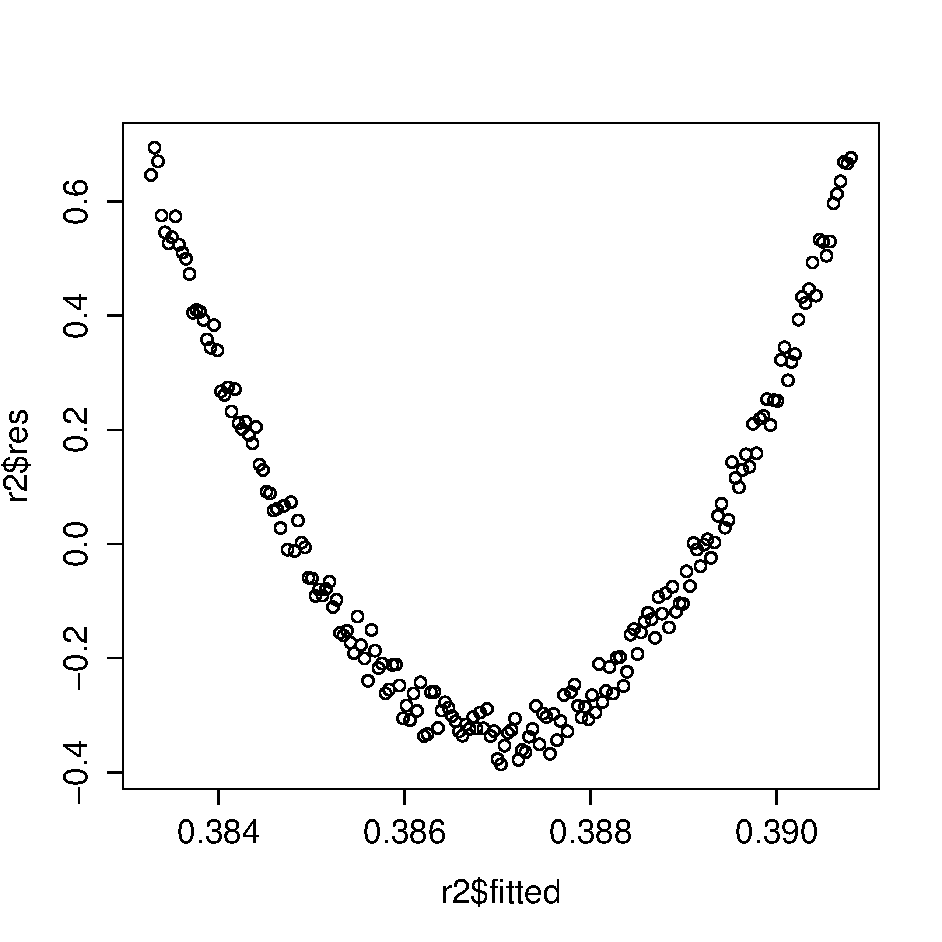
\includegraphics[scale=0.3]{nonadd.pdf}

\end{minipage}

\end{frame}

\begin{frame}{Additivitat i linealitat}
Quan es planteja un model lineal, les següents suposicions en són implícites:
\begin{itemize}
\item \emph{Additivitat}: Per cada variable independent $X_k$, la variació de $\mu_{Y|x_1,\ldots,x_k}$ associada amb un augment en $X_k$ (mantenint les altres variables constants) és la mateixa siguin quin siguin els valors de les altres variables independents.
\item \emph{Linealitat}:  Per cada variable independent $X_k$, la variació de $\mu_{Y|x_1,\ldots,x_k}$ associada amb un augment en $X_k$ (mantenint les altres variables constants) és la mateixa sigui quin sigui el valor de $X_k$.
\end{itemize}

Podem comprovar l'additivitat amb el test de Tukey, mentre que s'empraran els anomenats gràfics de residus parcials per la linealitat.

\end{frame}

\begin{frame}{Test de Tukey per la no additivitat}
La idea principal és verificar que no hi hagi interacció entre les variables independents i així, cada una tendrà un efecte additiu en el model. Si existeix la interacció, alguns termes quadràtics tendran pes en el model. Aquesta és la base del Test de Tukey.  
\begin{enumerate}
\item S'obtenen els $\{\hat{y}_i\}$ per la regressió lineal inicial.
\item Es duu a terme una segona regressió lineal incloent com a nova variable independent els $\hat{y}_i^2$. Sigui $\beta$ el coeficient d'aquesta nova variable.
\item Es realitza el contrast
$$\left\{\begin{array}{ll} H_0:  \beta=0\\ H_1: \beta\neq 0\end{array}\right.$$
Si no podem descartar la hipòtesi nul·la, la variable dels  $\hat{y}_i^2$ no és significativa i el model és additiu. 
\end{enumerate}

\end{frame}

\begin{frame}[fragile]{Test de Tukey per la no additivitat}
\begin{footnotesize}


\begin{verbatim}
> yhat2<-predict(r)^2
> rnova<-update(r,.~.+yhat2)
>  summary(rnova)
Call:
lm(formula = y ~ x + yhat2)
...
            Estimate Std. Error t value Pr(>|t|)    
(Intercept)  1.03464    0.03838  26.956   <2e-16 ***
x           -2.06595    0.05781 -35.735   <2e-16 ***
yhat2       -0.02653    0.05068  -0.524    0.602    
---
Sig. codes:  0 ‘***’ 0.001 ‘**’ 0.01 ‘*’ 0.05 ‘.’ 0.1 ‘ ’ 1
Res. standard error: 0.1671 on 97 degrees of freedom
Multiple R-squared:  0.9294,	Adjusted R-squared:  0.928 
F-statistic: 638.8 on 2 and 97 DF,  p-value: < 2.2e-16
\end{verbatim}
\end{footnotesize}
I amb un p-valor de 0.602, no podem rebutjar que el model sigui additiu.
\end{frame}

\begin{frame}[fragile]{Test de Tukey per la no additivitat}
Amb R, la funció \texttt{residualPlots} del paquet \texttt{car}, entre altres coses, retorna l'estadístic i el p-valor del Test de Tukey.

\begin{verbatim}
> residualPlots(r)
           Test stat Pr(>|t|)
x             -0.524    0.602
Tukey test    -0.524    0.601
\end{verbatim}

\end{frame}

\begin{frame}{Linealitat: Gràfics de residus parcials}

Els gràfics de residus parcials són una eina útil per detectar la no linealitat en una regressió. Es defineixen els \emph{residus parcials} $e_{ij}$ per la variable independent $X_j$ com
$$e_{ij}=e_i+b_jx_{ij}$$
on $e_i$ és el residu de la regressió lineal, $b_j$ és el coeficient de $X_j$ i $x_{ij}$ és l'observació $j$-èsima de l'individu $i$. 

\vspace{0.25cm}

Els residus parcials es dibuixen contra els valors de $x_j$ i es fa la seva recta de regressió. Si aquesta no s'ajusta a la corba donada per una regressió no paramètric suau (les variables independents no estan predeterminades i es construeixen amb les dades), el model no és lineal. 

\medskip

La funció de R per representar aquests gràfics és \texttt{crPlots} del paquet \texttt{car}.

\end{frame}

\begin{frame}[fragile]{Gràfics de residus parcials}
Anem a construir una variable més o manco lineal, una quadràtica i una altra logarítmica i facem-ne la regressió i els gràfics de residus parcials.

\begin{verbatim}
> y<-c(1:1000)
> x1<-c(1:1000)*runif(1000,min=0,max=2)
> x2<-(c(1:1000)*runif(1000,min=0,max=2))^2
> x3<-log(c(1:1000)*runif(1000,min=0,max=2))
> library(car)
> lm_fit<-lm(y~x1+x2+x3)
> crPlots(lm_fit)
\end{verbatim}

Com es pot veure als gràfics següents, les variables $x2$ i $x3$ no s'ajusten al model lineal. 

\end{frame}

\begin{frame}[fragile]{Gràfics de residus parcials}
\begin{center}
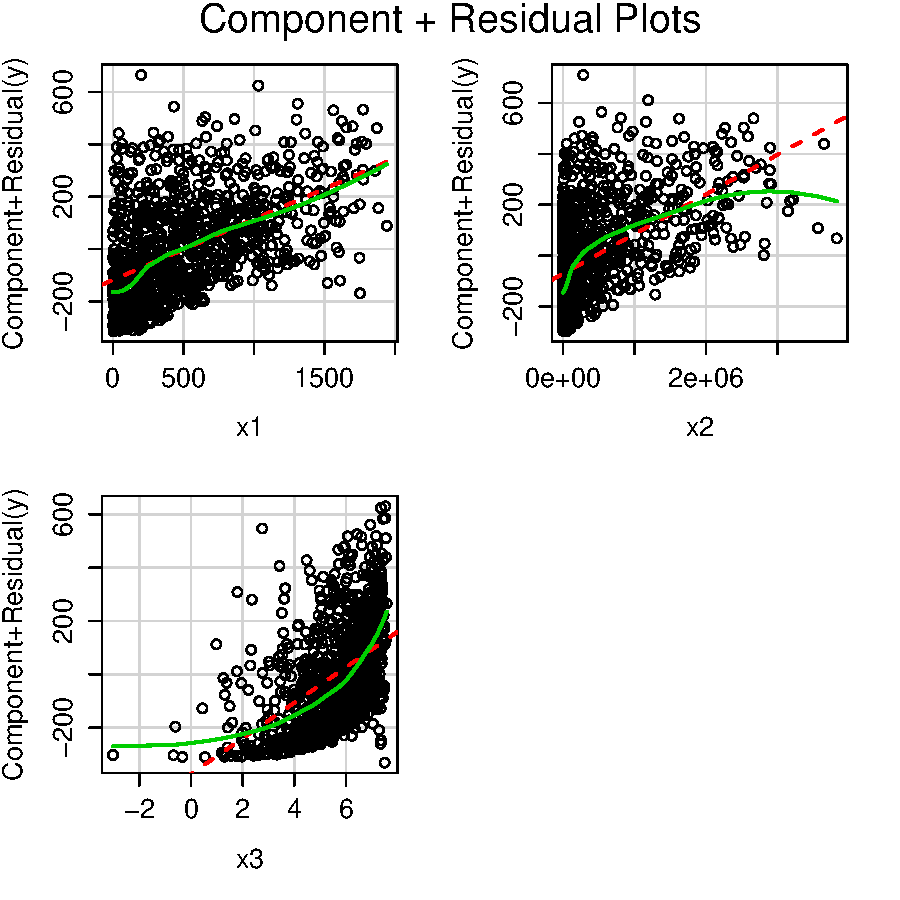
\includegraphics[scale=0.55]{crplot.pdf}
\end{center}
\end{frame}

\subsection{Observacions anòmales}
\begin{frame}{Observacions anòmales}
\begin{itemize}
\item Les observacions anòmales poden provocar que es malinterpretin patrons en el conjunt de dades.
\item A més, punts aïllats poden tenir una gran influència en el model de regressió donant resultats completament diferents.
\item Poden provocar que el nostre model no capturi característiques importants de les dades.
\end{itemize}
\end{frame}

\begin{frame}{Exemple}
\begin{center}
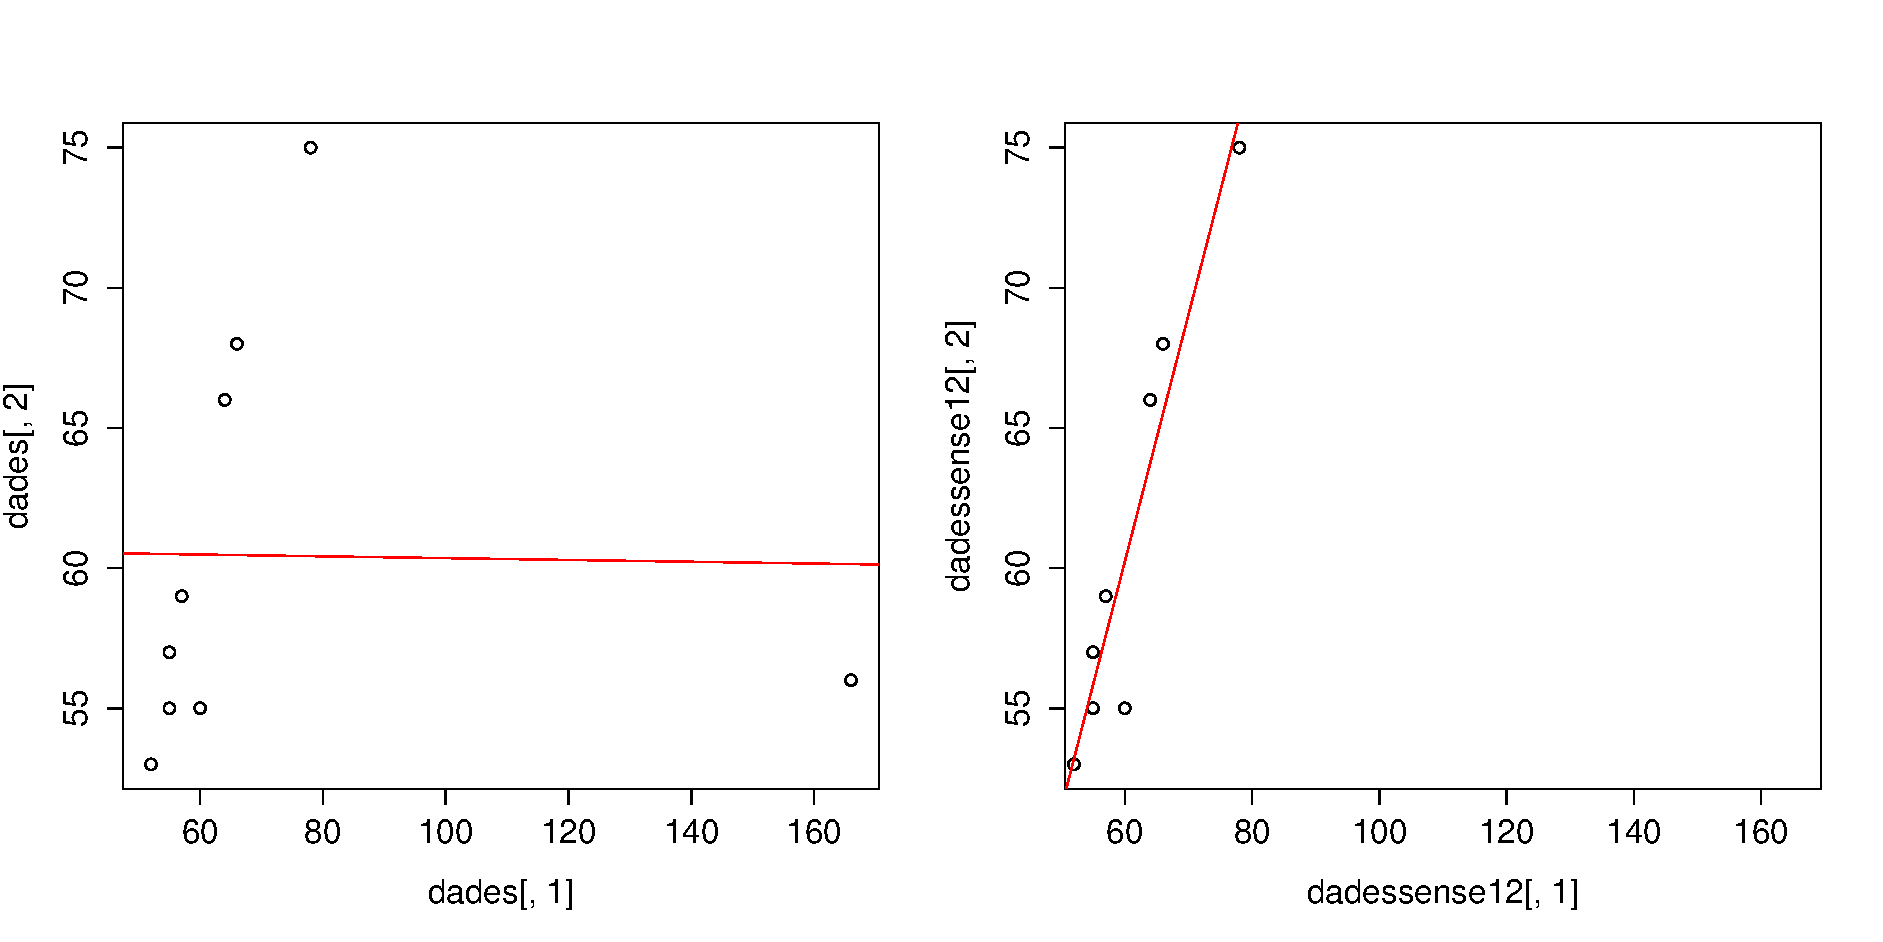
\includegraphics[scale=0.3]{outlier1.pdf}
\end{center}

Com es pot observar, la presència d'un valor anòmal distorsiona completament el model.

\end{frame}

\begin{frame}{Tipus d'observacions anòmales}

Tenim tres tipus d'observacions anòmales:
\begin{enumerate}
\item \emph{Outliers de regressió}: És una observació que té un valor anòmal de la variable dependent $Y$, condicionat als valors de les seves variables independents $X_i$. Tendrà un residu molt alt però pot no afectar massa al pendent.
\item \emph{Leverages}: És una observació amb un valor anòmal de les variables independents $X_i$. No té perquè afectar els coeficients de la regressió.
\item \emph{Observacions influents}: Són aquelles que tenen un alt leverage i són outliers de regressió i afecten fortament a la regressió.

\end{enumerate}

\end{frame}

\begin{frame}{Exemple}

\begin{center}
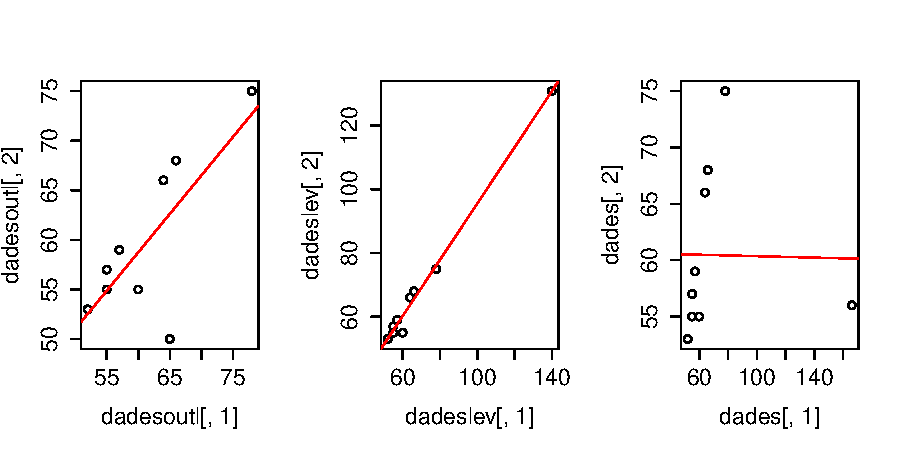
\includegraphics[scale=0.65]{tipus_anomal.pdf}
\end{center}
Aquestes seran les dades que emprarem a continuació. El primer data frame (dadesoutl) conté un outlier; el segon (dadeslev), un leverage i el tercer (dades), un punt influent.
\end{frame}

\begin{frame}{Leverages}
Per trobar els leverages, en primer lloc, anem a definir la \emph{ matriu Hat} $H$ donada per
$$H=X(X'X)^{-1}X'$$
Aquesta matriu és simètrica ($H^t=H$) i idempotent ($H^2=H$). A	més, és fàcil comprovar que $\hat{y}=Xb=X(X'X)^{-1}X'y=Hy$ i així tenim que
$$\hat{y}_{j}=h_{1j}y_1+h_{2j}y_2+\ldots+h_{nj}y_n=\sum_{i=1}^n{h_{ij}y_i}$$
\end{frame}

\begin{frame}{Leverages}

\begin{itemize}
\item Si $h_{ij}$ és gran, l'observació $i$-èsima té un impacte substancial en el valor predit $j$-èsim.
\medskip
\item Es defineix el \emph{leverage} de l'observació $i$-èsima, $h_i$ com el seu valor hat
$$h_i=\sum_{j=1}^n{h_{ij}^2}$$
i així, el valor hat $h_i$ mesura el leverage potencial de $y_i$ en tots els valors predits.
\end{itemize}

\end{frame}

\begin{frame}{Propietats leverages}

\begin{itemize}
\item El valor hat mitjà és $\overline{h}=\frac{k+1}{n}$.
\medskip
\item Els valors hat satisfan $\frac{1}{n}\leq h_i \leq 1$.
\medskip
\item En la regressió lineal simple, els valors hat mesuren la distància de $x_i$ a la mitjana de $X$:
$$h_i=\frac{1}{n}+\frac{(x_i-\overline{x})^2}{\sum_{j=1}^n{(x_j-\overline{x})^2}}$$
\medskip
\item En la regressió múltiple, $h_i$ mesura la distància d'una observació al vector de mitjà de $X$.
\end{itemize}
\end{frame}

\begin{frame}[fragile]{Leverages}

La regla de decisió és que es considerarà que una observació té leverage gran (i per tant, ha de ser considerada amb cura) quan $$h_i>2\frac{k+1}{n}.$$

La funció \texttt{hatvalues} de R calcula els valors hat donat un model de regressió.


\end{frame}


\begin{frame}[fragile]{Leverages}
\begin{footnotesize}

\begin{verbatim}
> n=length(dadeslev[,1])
> m=mean(dadeslev[,1])
> vhat=1/n+(dadeslev[,1]-m)^2/sum((dadeslev[,1]-m)^2)
> vhat
[1] 0.1164117 0.1265361 0.1375958 0.1466197 0.1626316 
[6] 0.1133304 0.1466197 0.1225744 0.9276806
> hatvalues(lm(dadeslev[,2]~dadeslev[,1]))
        1         2         3         4         5        
0.1164117 0.1265361 0.1375958 0.1466197 0.1626316 
        6         7         8         9 
0.1133304 0.1466197 0.1225744 0.9276806 
> which(vhat>2*2/n)
[1] 9
> dadeslev[9,]
        X        Y
91    140   130.77
\end{verbatim}

\end{footnotesize}
\end{frame}

\begin{frame}{Outliers}
\begin{itemize}
\item L'estratègia per determinar quines observacions són susceptibles de ser outliers es basen en els anomenats \emph{residus Studentitzats}. 
\item Es basen en recalcular el model després d'eliminar l'observació $i$-èsima i trobar la corresponent $(MSE)_i$.
\item Es defineixen com
$$E_i^\star=\frac{e_i}{\sqrt{(MSE)_i(1-h_i)}}$$
i segueixen una distribució $t$ d'Student amb $n-k-2$ graus de llibertat.
\end{itemize}
\end{frame}

\begin{frame}{Outliers}
\begin{itemize}
\item Es realitza una correcció de Bonferroni al p-valor multiplicant-lo per $n$ i així, el p-valor ajustat és
$$2nP(t_{n-k-2}\geq E_i^\star)$$ 
\item Es van considerant per ordre decreixent de $E_i^\star$ fins que es troba una observació que ja no sigui un outlier.
\end{itemize}
\end{frame}

\begin{frame}[fragile]{Outliers}
\begin{footnotesize}

\begin{verbatim}
> n=length(dadesoutl[,1])
> rout=lm(dadesoutl[,2]~dadesoutl[,1])
> residus=summary(rout)$res
> hats=hatvalues(rout)
> sigmes=c()
> for (i in 1:n)
{sigmes=c(sigmes,summary(update(rout,subset=-i))$sigma)}
> rstudents=residus/(sigmes*sqrt(1-hats))
> 2*length(dadesoutl[,1])*(1-pt(abs(rstudents),n-3))
         1          2          3          4          5 
4.31827408 4.75837310 5.94956512 6.40049712 8.40087400
          6          7          8          9   
 3.80527695 8.83857494 4.79294502 0.02148867
> dadesoutl[9,]
     V1   V2
9    65   50
\end{verbatim}
\end{footnotesize}
I tendríem que la novena observació seria un outlier.
\end{frame}

\begin{frame}[fragile]{Outliers}

La funció de R que realitza aquest test de detecció d'outliers és la funció \texttt{outlier.test} del paquet \texttt{car}. 

\begin{verbatim}
> outlier.test(lm(dadesoutl[,2]~dadesoutl[,1]))
   rstudent unadjusted p-value Bonferonni p
9 -5.026907          0.0023876     0.021489
\end{verbatim}
Arribant a la mateixa conclusió.

\end{frame}

\begin{frame}{Observacions influents: Distància de Cook}

\begin{itemize}
\item Com hem dit, una observació influent és aquella que combina discrepància amb leverage.
\item Una forma de determinar-les és examinar com canvien els coeficients de la regressió si s'elimina una observació en concret.
\item La mesura per avaluar aquest canvi és l'anomenada distància de Cook:
$$D_i=\frac{e^2_{S_i}}{k+1}\cdot\frac{h_i}{1-h_i}$$
on $h_i$ és el leverage i $e_{S_i}$ és l'anomenat residu estandaritzat, donat per
$$e_{S_i}=\frac{e_i}{\sqrt{MSE(1-h_i)}}.$$

\end{itemize}

\end{frame}

\begin{frame}{Distància de Cook}
\begin{itemize}
\item El primer factor mesura el grau de ser outlier mentre que el segon mesura el grau de leverage.
\item Una regla per determinar quines observacions són influents és
$$D_i>\frac{4}{n-k-1}.$$
\end{itemize}
\end{frame}

\begin{frame}[fragile]{Distància de Cook}
\begin{footnotesize}


\begin{verbatim}
> r=lm(dades[,2]~dades[,1])
> hats=hatvalues(r)
> resstd=r$res/(summary(r)$sigma*sqrt(1-hats))
> cooks=resstd^2/2*hats/(1-hats)
> cooks
           1            2            3            4   
71.193885062  0.036284611  0.038913392  0.003134472  
           5            6            7            8   
 0.018290844  0.093186308  0.065299277  0.045157990 
           9
 0.240848787
> dades[which(cooks>4/2),]
     V1    V2
1   166    56
\end{verbatim}
\end{footnotesize}
Concloem que l'observació 1 és influent en el model.
\end{frame}

\begin{frame}[fragile]{Distància de Cook}

Les distàncies de Cook es poden calcular emprant la funció \texttt{cooks.distance} del paquet \texttt{car} de R. 
\begin{footnotesize}
\begin{verbatim}
> cooks.distance(r)
           1            2            3            4   
71.193885062  0.036284611  0.038913392  0.003134472  
           5            6            7            8   
 0.018290844  0.093186308  0.065299277  0.045157990 
           9
 0.240848787
\end{verbatim}
\end{footnotesize}
\end{frame}

\begin{frame}{I què en feim amb les observacions anòmales?}
\begin{itemize}
\item El tractament de les observacions anòmales és força complex.
\item Es poden deure a errors en l'entrada o recollida de les dades i en aquest cas, es podrien eliminar.
\item Però també poden explicar que no s'ha considerat alguna variable independent que afecta al conjunt d'observacions anòmales.
\item Les més perilloses són les influents. En el cas que es determini que es poden eliminar, s'han d'eliminar d'una a una, actualitzant el model cada vegada.
\end{itemize}


\end{frame}

\begin{frame}
\frametitle{Algunes consideracions finals: Selecció del model}
\begin{itemize}

\item El model de regressió lineal no és l'únic que podem emprar (polinòmics, logarítmics), i altres models podrien donar ajustaments millors
\medskip

\item El model pot ser més eficaç si afegim altres variables, o pot ser igual d'eficaç si llevam variables redundants
\medskip

\item Hi pot haver dependències lineals entre les variables que les faci redundants: ho podem detectar amb la matriu de covariàncies
\medskip

\item Hi ha mètodes iteratius per cercar el model lineal amb un millor equilibri de simplicitat i adequació: millor fer-los amb R
\end{itemize}

\end{frame}





\end{document}
